\chapter{Mechanik deformierbarer K"orper}
\label{kap_mechanik-deformierbarer-korper}




Bisher hatten wir zwischen zwei Teilchen eines K"orpers starre
Verbindungen angenommen. Unsere Neuen Grundannahmen sind:

\paragraph{Bindungstypen zwischen Atomen}
\label{kap_bindungstypen-zwischen-atomen}

\begin{description}[\setlabelstyle{\bfseries\slshape}]
\item[\index{Ionische Bindung}Ionische] Bindungen: Durch die
   \emph{\textsc{Coulomb}-Kraft} werden geladene Teilchen angezogen
   und abgesto"sen. So h"alt bspw. $\operatorname{NaCl}$ zusammen.
\item[\index{kovalente Bindung}kovalente] Bindungen: Durch
   elektrostatische Wechselwirkungen werden nicht-ionische
   (Nichtmetall-)Atome und andere Teilchen zusammengehalten -- so bspw
   auch $\operatorname{H_2}$.
\item[\textsc{\index{Van-der-Waals-Kr"afte}Van-Der-Waals}]-Kr"afte:
   Durch Quantenmechanische Effekte halten neutrale Teilchen
   aneinander -- bspw. $\operatorname{Ar}$-Atome
\end{description}
Wir denken uns Festk"orper als Stoffe, die aus Atomen bestehen, die
\emph{feste} Pl"atze einnehmen. Die Atomen sind entweder geordnet und
bilden \textbf{\index{Kristalle}Kristalle} oder ungeordnet -- dann
hei"st der K"orper \textbf{\index{amorph}amorph} und wir bezeichnen
ihn als "`\textbf{\index{Glas}Glas}"'.


\paragraph{Erw"armung}
\label{kap_erwarmung}

Die Atome haben zwar eine Feste Position im Festk"orper, jedoch ist
dieser eigentlich nur eine \emph{Gleichgewichtslage}; sie k"onnen um
diesen herum \emph{Schwingungen} ausf"uhren.

Beim Erw"armen werden diese Schwingungen st"arker. "Uberhalb einer
kritischen Temperatur werden die Schwingungen so stark, dass sie die
Bindungskr"afte "uberwinden k"onnen und der Festk"orper so zerst"ort
wird. Das kennen wir als \textbf{\index{Schmelzen}Schmelzen}.


\paragraph{Festk"orper vs Fl"ussigkeiten}
\label{kap_festkorper-vs-flussigkeiten}

In Fl"ussigkeiten sind Atome gegeneinander verschiebbar d.h. sie haben
keinen Festen (Gleichgewichts-)Punkt und somit auch \emph{keine
  Formstabilit"at}. Dennoch ist die Dichte einer Fl"ussigkeit mit der
von Festk"orpern vergleichbar.

Beim Erw"armen schwingen auch hier die Atome schneller und wenn hier
die Kr"afte "uberwunden werden, die die Fl"ussigkeitsteilchen
zusammenhalten, so \textbf{\index{Verdampfen}verdampft} der Stoff.








\section{Deformierbare Festk"orper}
\label{kap_deformierbare-festkorper}


Wir n"ahren das Potential der Bindung zweier Atome mit dem Potential
einer Feder an. Dies ist eine N"ahrung, die nur in einem rechtkleinen
Bereich funktioniert. Das liegt daran, dass das Potential bei Atomen
in Kernn"ahe mit $V \sim \frac{1}{x^2}$ beschrieben wird und weiter
entfernt mit $V \sim -\frac{1}{x}$. Bei der Feder hingegen wird das
Potential nach $E_{spann} = \frac{1}{2}D \, \Delta x^2$ beschrieben
mit $V \sim (x-x_0)^2$. In Abb. \ref{abb_atompotential-federpotential}
ist Realit"at und N"ahrung\footnote{Also ein Potential $V =
  \frac{A}{x^2} - \frac{B}{x}$ mit weigehend beliebigen (positiven)
  $A$ und $B$ und eine Kurve mit $V_D = C\cdot (x-x_0)^2$ bei dem $C$
  und $x_0$ (m"oglichst) genau angepasst wurden. Dies gibt den Verlauf}
verglichen. \footnote{"Ubrigens ist dieses Atompotential ein
  Ausschnitt des Potentials in Abb. \ref{abb_kristallpotential}.}


Steigt die Temperatur im Feststoff an, so schwingen die Atome st"arker
um ihre Ruhelage. Im Diagramm hei"st das, dass sie eine h"ohere Energie
haben (also auf einem h"oheren Potential liegen, also im Schaubild
\emph{h"oher} sind) und damit weiter nach rechts (also weg vom Kern)
ausschwingen k"onnen, weil hier die Kurve f"ur das Potential im Atom ja
flacher wird. F"ur diesen Fall m"ussen wir eigentlich eine neue Parabel
anpassen, deren Mittelpunkt weiter nach rechts verschoben ist, um die
neue Situation besser zu modellieren


\begin{figure}
   \centering
   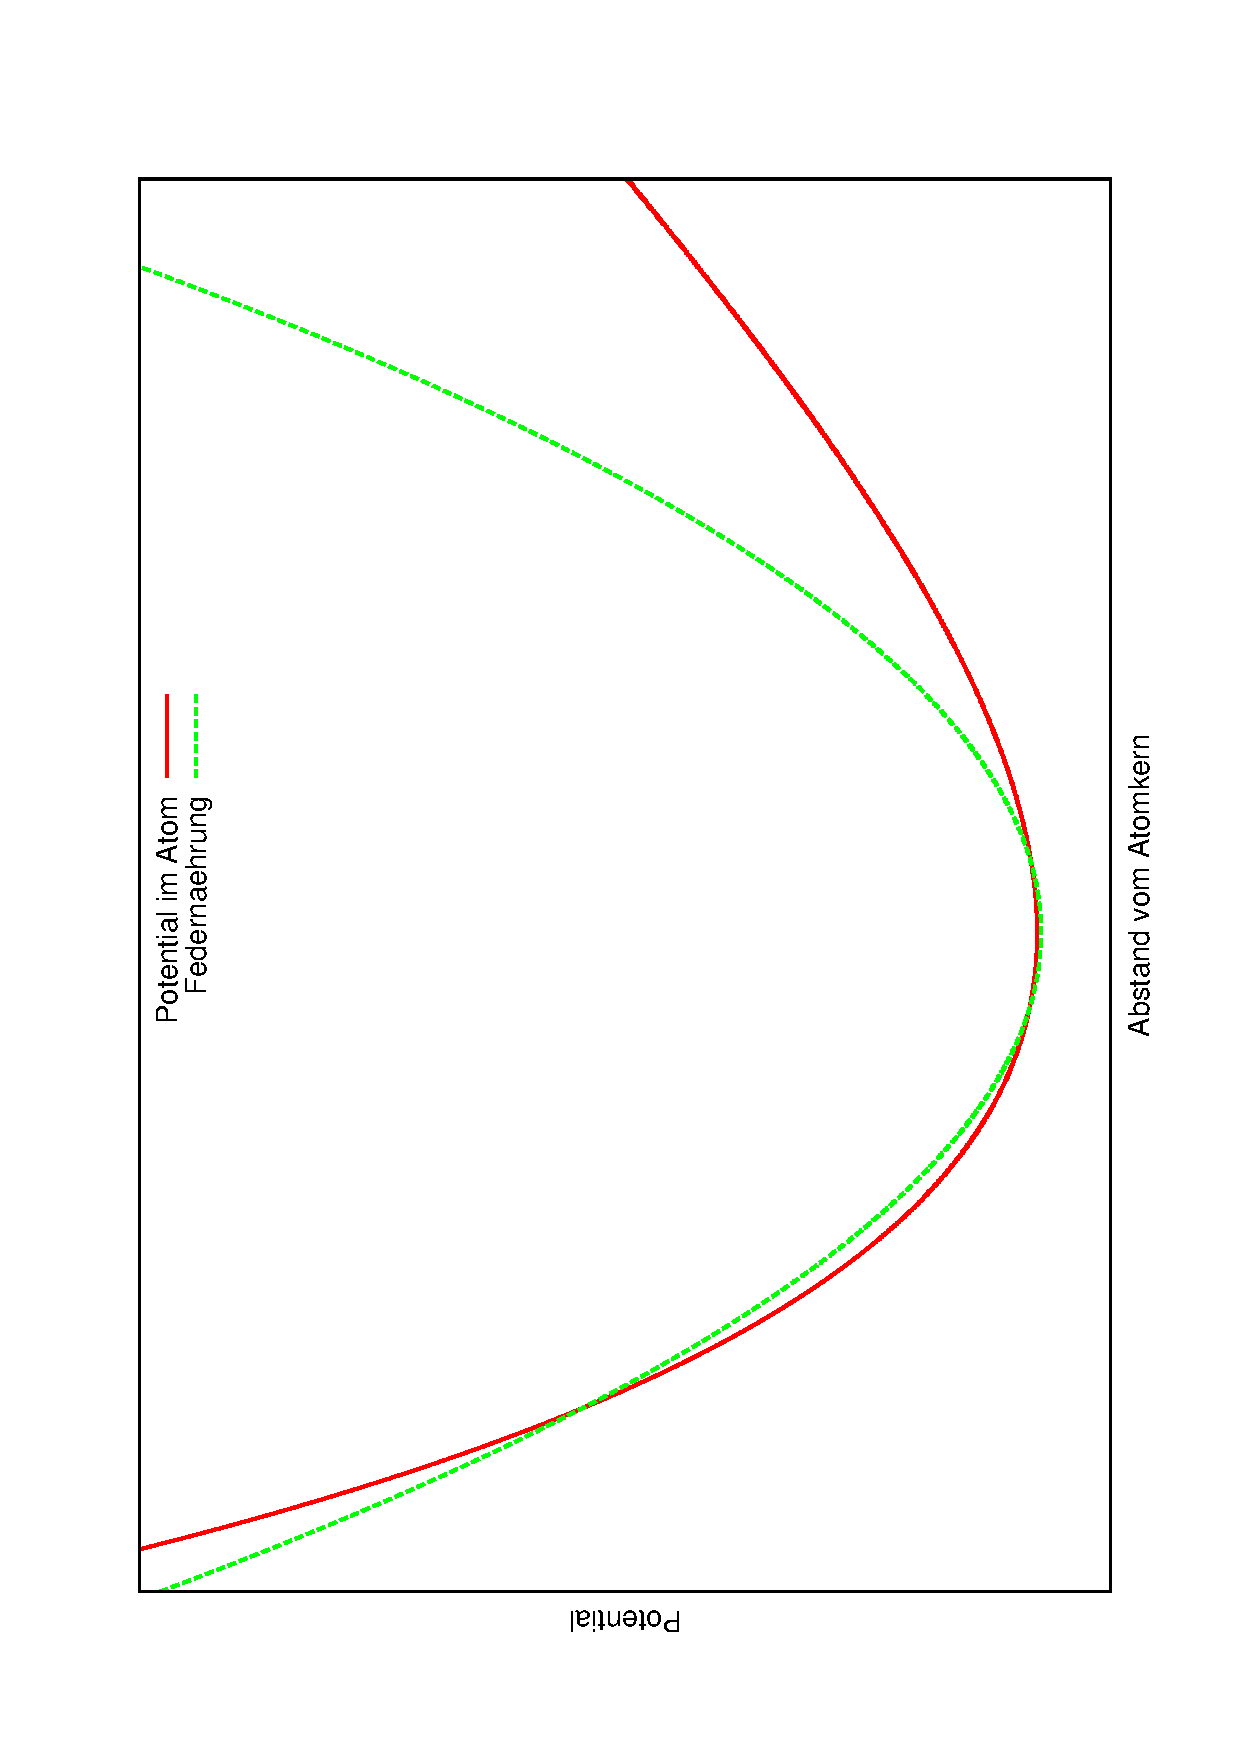
\includegraphics[width=0.7\textwidth,angle=-90]{bilder/atompot}
   \caption[Potentiale: Atomar, Feder]{Potential im Atom im Vergleich
     mit dem quadratischen Potential einer Feder}
   \label{abb_atompotential-federpotential}
\end{figure}

Wir verwenden diese Feder-N"aherung also im zul"assigen Bereich -- dort
wo sich in Abb. \ref{abb_atompotential-federpotential} die Kurven
weitestgehend "uberlappen -- und f"uhren das \textbf{Federmodell} ein.


\begin{Def}
   [\index{Federmodell}Federmodell]
Im Federmodell betrachten wir einen Festk"orper als punktf"ormige
Massen, die durch Federn verbunden sind.
\end{Def}



Mit diesem Modell k"onnen wir folgern, dass Festk"orper innerhalb
gewisser Grenzen \textbf{elastisch verformbar} sind:
\begin{Def}
   [\index{Elastisch}Elastisch verformbar]
Der K"orper ver"andert seine Form, wenn eine Kraft auf ihn ausge"ubt
wird, nimmt seine alte Form aber wieder an, wenn die angreifenden
Kr"afte verschwinden.
\end{Def}

Weil wir au"serdem die Parabel bei h"oheren Temperaturen nach rechts
verschieben m"ussen, bekommen die Ruhelagen der Atome einen gr"o"seren
Abstand zwischeneinander und somit \emph{expandiert} der K"orper
dann. Wir sprechen hier von einer \textbf{\index{thermische
    Expansion}thermische \index{Expansion, thermische}Expansion}.



\section{Kr"afte auf Festk"orper}
\label{kap_krafte-auf-festkorper}


\subsection{Dehnung}
\label{kap_dehnung}

Wir ziehen an dem Werkstoff der L"ange $L$ mit der Kraft $F$ (parallel
zu $L$) und dehnen ihn dadurch \textbf{absolut} um die Strecke $s$
bzw. Dehnung $\Delta L$ aus oder relativ um die
\textbf{\index{relative Dehnung}relative Dehnung} $\varepsilon =
\frac{\Delta L}{L}$. 


In Abb. \ref{abb_dehnung} ist eine Kurve einer typischen
Dehnung aufgetragen. Hier sieht man die verschiedenen staden
reversibler und irreversibler Verformung.

\begin{figure}
   \centering
   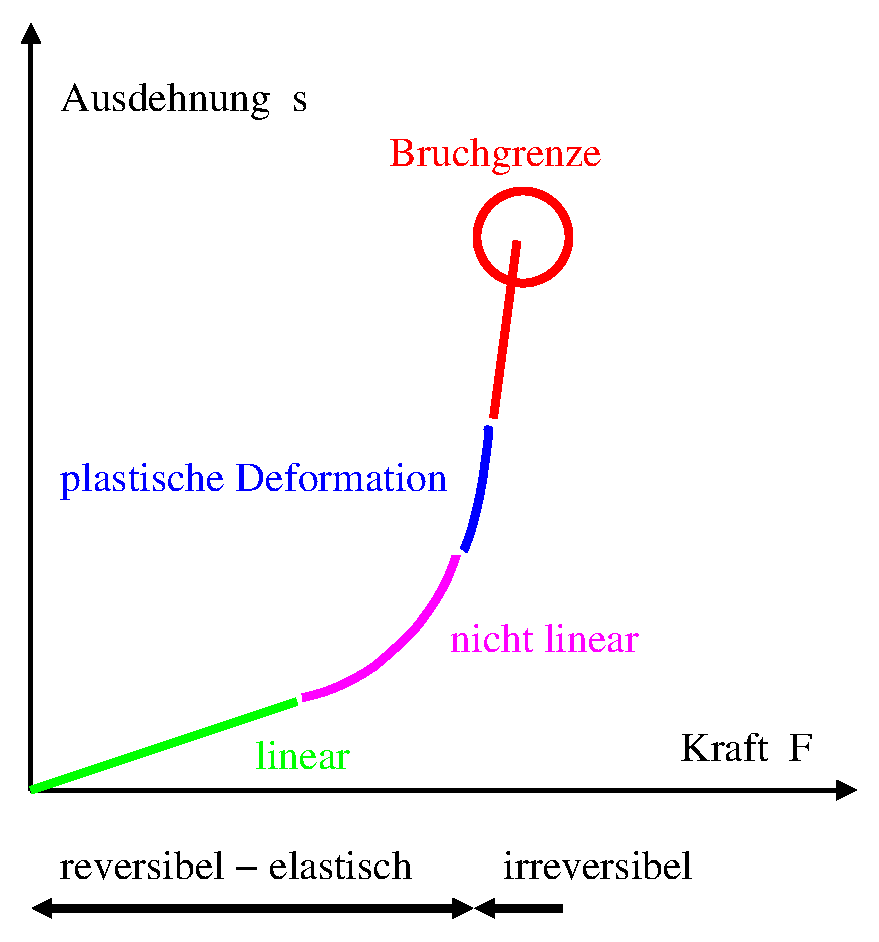
\includegraphics[width=0.7\textwidth]{bilder/dehnung}
   \caption{Dehnung eines Feststoffs im $s$-$F$-Diagramm}
   \label{abb_dehnung}
\end{figure}

Wir unterscheiden die angreifenden Kr"aften danach, wie sie angreifen;
entweder senkrecht zur K"orperoberfl"ache
oder waagerecht dazu. Wir wollen uns hier mit den Kr"aften
\emph{senkrecht} zur Oberfl"ache befassen:
\begin{Def}
   [\index{Zugspannung}(Zug-/\index{Druckspannung}\index{Spannung}Druck)Spannung
   \emph{"`\index{Stress"'}Stress"'} $\sigma$] Die Kraft ($\vec F_N$)
   zeigt senkrech ("`normal"') zur Oberfl"ache $A$ des K"orpers
\begin{equation}
   \label{eqn_Def_zugspannung}
   \sigma = \frac{\|\vec F_N\|}{A}
\end{equation}
\end{Def}
mit $[\sigma] = \frac{\operatorname{N}}{\operatorname{m^2}} = Pa =
10^{-5} \operatorname{bar}$


\bigskip

F"ur \textbf{kleine Amplituden} gilt f"ur die Verformung $\Delta L$ eines
K"orpers der L"ange $L$: 
$$
\Delta L \sim F \text{ , \;  } \Delta L \sim L \text{ und } \Delta L \sim \frac{1}{A}
$$
und so definieren wir:
\begin{Def}
   [\index{Elastizit"atsmodul}Elastizit"atsmodul $E$]
Eine \emph{Materialkonstante} f"ur die gilt
\begin{equation}
   \label{eqn_der_elastizitaetsmodul}
   E = \frac{\sigma}{\varepsilon} = \frac{F \cdot  L}{A \cdot \Delta
     L} ~ ~ \Leftrightarrow ~ \boxed{ \sigma = E \cdot \varepsilon }
\end{equation}
\end{Def}
Dieser Zusammenhang wird auch als \textbf{\textsc{Hook}'sches Gesetz}
bezeichnet. Vergleiche Dazu die \emph{Federh"arte} $D = \frac{F}{\Delta
L}$; 

\begin{quote}
   Je gr"o"ser $E$ ist, desto schwerer ist es -- also desto mehr Kraft
   $F$ muss man aufbringen -- um den K"orper um $\Delta L$ zu
   verformen.
\end{quote}


\emph{Eigentlich} m"ussten wir aber $E$ definieren als 
\begin{equation}
   \label{eq:55}
   E = \frac{\diff \sigma}{\diff \varepsilon}
\end{equation}
Nur weil wir im Bereich der linearen Expansion arbeiten
(s. Abb. \ref{abb_dehnung}) d"urfen wir die Definition oben verwenden.

\bigskip

\noindent
Wenn wir einen K"orper strecken, so werden wir beobachten, dass er
seinen Querschnitt verkleinert -- dies bezeichnet man als
\textbf{\index{Querkontraktion}Querkontraktion}. Man kann sie dadurch
erkl"aren, dass der K"orper bestrebt ist, sein Volumen gleich zu
halten.

Es gilt dabei -- wieder f"ur kleine Verformungen -- wenn wir eine
Querschnittsfl"ache mit $A = d^2$ annehmen (also $V = L\cdot d^2$):
Auch wenn der K"orper \emph{versuchen} mag, sein Volumen konstant zu
halten, so "andert es sich doch. Zieht man in L"angsrichtung an dem
K"orper, so verl"angert er diese Seite um $\Delta L$ ($\Delta L > 0$),
gleichzeitig werden sich die anderen Seiten $d$ verk"urzen ($\Delta d <
0$). Wir k"onnen f"ur die neuen L"angen also $L' = L + \Delta L$ und $d'
= d + \Delta L$ schreiben, und bekommen,
% $$
% V' = (d - \Delta d)^2 \cdot (L - \Delta L) = \underbrace{d^2 L}_V -
% 2d\Delta d \cdot L + (\Delta d)^2 \cdot L - d^2 \cdot \Delta L + 2 d
% \Delta d \cdot \Delta L - (\Delta d)^2 \cdot \Delta L
% $$
wenn wir in gewohnter Manier alle Therme streichen, die ein
quadratisches oder zwei verschiedene $\Delta$  enthalten:
$$
V' \approx V + 2d\Delta d L + d^2 \cdot \Delta L
$$
und weiter
$$
\Delta V \approx  d^2 \cdot \Delta L + 2d\Delta d L
$$
teilt man dies durch $V = d^2 \cdot L$ ergibt sich:
\begin{equation}
   \label{eq:56}
   \frac{\Delta V}{V} \approx \frac{\Delta L}{L} + 2 \frac{\Delta
     d}{d} = \varepsilon + 2 \varepsilon_q
\end{equation}
Dabei haben wir die \textbf{\index{relative Querkontraktion}relative
  \index{Querkontraktion}Querkontraktion $\varepsilon_q = \frac{\Delta
    d}{d}$} eingef"uhrt.  Das Verh"altnis zwischen (relativer)
Querkontraktion $\varepsilon_q$ und (relativer) Dehnung $\varepsilon$
bezeichnet man mit der \textbf{\index{Poissonzahl}Poissonzahl} oder
\textbf{\index{Querkontraktionszahl}Querkontraktionszahl}\footnote{Das
  "`$-$"' ist da, weil eine der beiden Kontraktionen $\varepsilon$
  oder $\varepsilon_q$ (praktisch) immer negativ ist, wenn die andere
  positiv ist -- dadurch erh"alt man ein positives $\mu$.}
\begin{equation}
   \label{eqn_def_poissonzahl}
   \mu = - \frac{\frac{\Delta d}{d}}{\frac{\Delta L}{L}} =
- \frac{\varepsilon_q}{\varepsilon} =
-   \frac{\Delta d \cdot L}{d \cdot \Delta L}
\end{equation}
und man erh"alt in Gl. \eqref{eq:56} durch Einsetzen:
\begin{equation}
   \label{eq:57}
   \boxed{\frac{\Delta V}{V} \approx \frac{\sigma}{E} ( 1 - 2\cdot \mu) }= (1
   - 2\mu) \cdot \varepsilon
\end{equation}


Im Allgemeinen ist 
$$
\Delta V < 0 ~ \Leftrightarrow ~ \mu > 0
$$
Es gibt aber auch bestimmte Stoffe, bei denen $\mu < 0$ ist -- der
Stoff wird also beim Ziehen l"anger \emph{und} breiter.




\subsection{Kompression}
\label{kap_kompression}


Wirkt eine \textbf{Kraft von allen Seiten} auf den K"orper, so hat er
keine andere M"oglichkeit, sich zu verformen und sein Volumen zu
verringern. 

Bei einem Druck $p$ -- f"ur den nach Definition $p = - \sigma$
gilt\footnote{Bei der Spannung $\sigma$ wirkt die Kraft nach au"sen,
  der Druck $p$ wirkt von au"sen auf den K"orper.} -- verk"urzt sich
eine Seite nach \eqref{eqn_der_elastizitaetsmodul} und mit $p =
\frac{F}{A}$ um $\Delta L = L \frac{\sigma}{E} = - L \frac{p}{E}$. Die
Seitenfl"achen mit L"ange $d$ w"urden sich eigentlich um $\Delta d = -
d \frac{p}{E}$ verk"urzen -- durch die Verk"urzung von $L$ muss $d$
sich aber noch zus"atzlich um $\Delta d = - \mu \frac{ \Delta L
  }{L} d = - \mu \cdot \frac{p}{E} \cdot d$ "andern. Diese zweite
"Anderung m"ussen wir auch noch doppelt gewichten, % weil sich eine
% Seite verl"angert, wenn eine andere sich verk"urzt -- in diesem
% 3-D-K"orper, auf den von allen Seiten Druck wirkt, "andern sich immer
% alle drei Seiten, also verk"urzen sich \emph{zwei} der anderen Seiten,
% wenn sich $d$ verl"angert.
%% neu folgt
weil die "Anderung einer der Kantenl"angen sich auf die "Anderung von
\emph{zwei} Kanten auswirkt -- und umgekehrt wirken auf die "Anderung
einer Kantenl"ange \emph{zwei} andere Kantenl"angen ein.

Diese Argumentation k"onnen wir f"ur jede der drei Seitenl"angen $\ell_i$ getrennt
durchf"uhren und kommen stets auf das selbe
Ergebnis:\footnote{Alternativ: Eine Seite verk"urzt sich um
  $\varepsilon = \frac{\sigma}{E}$ und so folgt f"ur eine beliebige
  andere $\varepsilon' = \varepsilon_q = - \mu \varepsilon = - \mu
  \frac{\sigma}{E}$. Eine Seite ver"andert sich also um $\varepsilon +
  2 \varepsilon'$ (die beiden gestrichenen Terme kommen von der
  Kontraktion der jeweils anderen Seiten) und so folgt
  $\varepsilon_\text{ges} = \frac{\sigma}{E} - 2 \mu \frac{\sigma}{E}$.}
\begin{equation}
   \label{eq:58}
   \Delta \ell_i = - \ell_i \cdot \frac{p}{E} ( 1 - 2 \mu)
\end{equation}
Wenn wir nun das Volumen mit Gl. \eqref{eq:56} berechnen wollen, so
vernachl"assigen wir wieder wie oben alle Terme mit mehreren $\Delta$s
und erhalten\footnote{Hier ist wichtig, dass die Poissonzahl $\mu$
  diesmal ein negatives Vorzeichen hat, weil sowohl $\varepsilon$ als
  auch $\varepsilon_q$ negativ sind!}
\begin{equation}
   \label{eq:59}
   \frac{\Delta V}{V} = \frac{\Delta L}{L} + 2 \frac{\Delta d}{d} =
   -3\frac{p}{E} (1 - 2 \mu) = - \frac{1}{K} \Delta p = - \kappa \cdot
   \Delta p
\end{equation}
Wobei wir definiert haben:
\begin{Def}
   [\index{Kompressionsmodul}Kompressionsmodul $K$, \index{Kompressibilit"at}Kompressibilit"at $\kappa$]
   \begin{equation}
      \label{eqn_def_kompressionsmodul}
      \kappa = \frac{1}{K} = - \frac{1}{\Delta p} \frac{\Delta V}{V} =
      \frac{3}{E}(1 - 2\mu) 
% \text{ bzw. } ~ \kappa \cdot \Delta p = -
%       \frac{\Delta V}{V}
\text{ bzw. } \boxed{\Delta p = - K\frac{\Delta V}{V}}
   \end{equation}
\end{Def}
Das Kompressionsmodul beschreibt also, welcher Druck n"otig ist, um
eine bestimmte relative Volumen"anderung hervorzurufen. Die
Kompressibilit"at zeigt den proportionalen Zusammenhang zwischen
Druck"anderung und relativer Volumen"anderung.




\subsection{Scherung}
\label{kap_scherung}

Analog zur Druckspannung senkrecht auf die Oberfl"ache eines K"orpers,
kann auch die Schubspannung $\vec F_T$  \emph{\textbf tangential} zur
Oberfl"ache wirken:

\begin{Def}
   [\index{Schubspannung}Schub/-\index{Scherspannung}Scherspannung $\tau$]
Die Kraft ($\vec F_T$) wirkt parallel der Oberfl"ache $A$ eines K"orpers
\begin{equation}
   \label{eqn_def_schubspannung}
   \tau = \frac{\|\vec F_T\|}{A}
\end{equation}
\end{Def}
mit der der Einheit $[\tau] = [\sigma] = \operatorname{Pa}$.

Nun untersuchen wir auch nicht mehr die "Anderung der Seitenl"ange,
sondern den sog. \textbf{\index{Scherungswinkel}Scherungswinkel}
$$
\alpha = \arctan \frac{\Delta L}{L}
$$

\begin{figure}
   \centering
   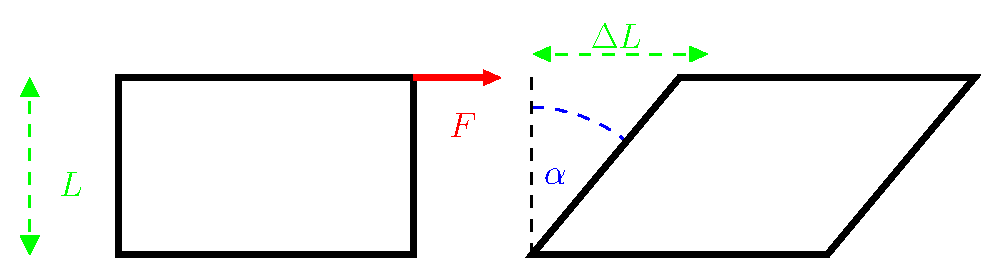
\includegraphics[width=0.7\textwidth]{bilder/scherung}
   \caption{Scherung eines K"orpers}
   \label{abb_scherung}
\end{figure}
Da f"ur kleine $x$ gilt\footnote{Der Taylor von Arctan um
  $0$: $$x-\frac{{x}^{3}}{3}+\frac{{x}^{5}}{5}-\frac{{x}^{7}}{7}+O(x^9)
  \text{ vgl Arcsinus: }
x+\frac{{x}^{3}}{6}+\frac{3\,{x}^{5}}{40}+\frac{5\,{x}^{7}}{112}+O(x^9)
$$}
$\arctan x \approx x$, setzten wir entsprechend
f"ur kleine Scherungen
\begin{equation}
   \label{eq:60}
   \alpha \approx \frac{\Delta L}{L}
\end{equation}
und definieren analog zum Elastizit"atsmodul:
\begin{Def}
   [\index{Schubmodul}Schubmodul $G$]
   \begin{equation}
      \label{eqn_def_schubmodul}
      G = \frac{\tau}{\alpha} ~ ~ \Leftrightarrow ~\boxed{\tau = G \cdot \alpha}
   \end{equation}
\end{Def}

Zwischen den Moduln $E$, $K$ und $G$ gilt im Allgemeinen:
\begin{equation}
   \label{eq:62}
   \boxed{
\frac{E}{2G} = 1 + \mu
} 
\text{ und }
\boxed{
\frac{E}{3K} = 1 - 2\mu
}
\end{equation}


Da bei einer Stauchung die Bindungs\emph{winkel} gleich bleiben, bei
einer Scherung dagegen die Bindungs\emph{l"angen}, und die jeweils
anderen Gr"o"sen sich ver"andern, brauchen wir die beiden Moduln:
\begin{Wichtig}
Ein K"orper reagiert im Allgemeinen verschieden darauf, ob er gedehnt oder
geschert wird...   
\end{Wichtig}




\section{Ruhende Fl"ussigkeiten}
\label{kap_ruhende-flussigkeiten}


\subsection{Oberfl"ache}
\label{kap_oberflache}


Die Teilchen einer Fl"ussigkeit k"onnen sich frei bewegen -- somit ist
ihre \emph{Position} logischwerweise nicht fest bestimmt. Bei der
\emph{Oberfl"ache} ist es jedoch anders: 
\begin{Wichtig}
Eine Fl"ussigkeitsoberfl"ache ist (nach einiger Zeit) immer senkrecht
  zur Summe aller einwirkenden Kr"afte.
\end{Wichtig}
W"are dies \emph{nicht} so, so w"urden die Teilchen an der Oberfl"ache
der Kraft folgen -- also in Richtung Kraft flie"sen. Dieses Verhalten
w"urde sich erst einstellen, wenn alle Fl"ussigkeitsteilchen auf einer
\emph{"Aquipotentialfl"ache} der angreifenden Kr"afte liegen, weil dann
keines mehr dazu neigt, seine Energie durch Bewegung im Potential zu
minimieren. 

\begin{Wichtig}
   In Fl"ussigkeiten verschwindet das Schermodul $G$.
\end{Wichtig}




\subsection{Stempeldruck}
\label{kap_oberflache-1}


Bei den \emph{Kr"aften auf eine Fl"ussigkeit} spricht man i.A. von
\textbf{Druck}.

\begin{Def}
   [\index{Stempeldruck}Stempeldruck]
Die Kraft $F$ wirkt senkrecht auf eine Fl"ussigkeitsoberfl"ache $A$,
dann gilt:
   \begin{equation}
      \label{eqn_def_druck}
      p = \frac{F}{A}
   \end{equation}
\end{Def}
mit der Einheit $[p] = \frac{\operatorname{N}}{\operatorname{m^2}} =
Pa$.

Den Druck kennen wir schon aus dem Zusammenhang mit der Kompression
eines Festk"orpers \eqref{eqn_def_kompressionsmodul}:
$$
\frac{\Delta V}{V} = -\kappa \cdot \Delta p
$$
Tabelle \ref{tab_kompressibilitaeten_fluessigkeit} zeigt, dass man in
guter N"aherung behaupten kann, dass:
\begin{Wichtig}
   Fl"ussigkeiten sind inkompressibel
\end{Wichtig}


\begin{table}
   \centering
   \begin{tabular}{l c}
      \toprule
\textbf{Stoff} & Kompressibilit"at $\kappa$ in
$\frac{1}{\operatorname{Pa}}$\\
\midrule
Wasser (bei $20^\circ\operatorname{C}$) & $46 \cdot 10^{-11}$\\
Eisen & $6.6 \cdot 10^{-11}$\\
Stickstoff & $1 \cdot 10^{-5}$\\
\bottomrule
   \end{tabular}
   \caption{Kompressibilit"aten von \emph{Fl"ussigkeiten}}
   \label{tab_kompressibilitaeten_fluessigkeit}
\end{table}




\subsection{Schweredruck}
\label{kap_schweredruck}



W"ahrend der Stempeldruck an jeder Stelle gleich wirkt, ist der
Schweredruck an verschiedenen Stellen verschieden. Er resultiert aus
der Gewichtskraft, die Teilchen weiter oben in der Fl"ussigkeit nach
unten aus"uben.

\begin{Def}
   [\index{Schweredruck}Schweredruck]
Die Fl"ussigkeitss"aule "uber einem Teilchen im Wasser erzeugt den Druck
\begin{equation}
   \label{eqn_schweredruck}
p = \int_0^h \frac{\diff F}{A} =
 \int_0^h \frac{g \cdot \diff m}{A} =
 \int_0^h \frac{g \cdot \varrho \cdot A \cdot \diff z}{A} =
\boxed{\varrho \cdot g \cdot h = p}
\end{equation}
\end{Def}
Und dabei gilt:
\begin{Wichtig}
   Der Schweredruck ist unabh"angig von der Fl"ache $A$.
\end{Wichtig}

Es kann auch vorkommen, dass die Dichte einer Fl"ussigkeit nicht
konstant ist. Bspw. wenn die Temperatur in verschiedenen Bereichen
verschieden ist, ist die Dichte im warmen Bereich \emph{kleiner}.
\begin{Wichtig}
   $$\varrho = \varrho(\vec r)$$
\end{Wichtig}
Siehe dazu Kap. \ref{kap_ruhende-gase}.


\subsection{Kommunizierende R"ohren}
\label{kap_kommunizierende-rohren}

% Wenn wir Rohre beliebig so befestigen, dass wenn man in eines Wasser
% sch"uttet, es \emph{nicht} aus dem System l"auft, sonder sich darin
% verteilt, so ist in allen R"ohren, die miteinander verbunden sind --
% und bei denen diese Verbindung auch unter Wasser steht -- der
% Wasserpegel gleich.

In ein beliebiges Rohrsystem wird Wasser gegeben. Wenn zwei R"ohren
miteinander verbunden sind, und das Wasser erreicht diese Verbindung,
so wird es durch diese Verbindung hindurchgedr"uckt: "uber dem einen
Rohr steht eine Wassers"aule, und mit diesem Druck werden die
Wasserteilchen in die n"achst Rohre gedr"uckt. Sie steigen aber dort nur
so hoch dass die Kr"afte auf die Teilchen in den S"aulen gerade
ausgeglichen sind. Nach Gl. \eqref{eqn_schweredruck} ist dies nur
m"oglich, wenn die Wasserpegel gleich hoch sind (eine konstante Dichte
angenommen). 

Dabei ist nur die \emph{H"ohe} entscheidend, weil in unserem Beispiel nur die
Schwerkraft eine \emph{Kraft} nach unten aus"ubt, die nach $F = m \cdot
a$ f"ur eine Bewegung ben"otigt wird.

\begin{Wichtig}
   [Prinzip der \index{Kommunizierende R"ohren}Kommunizierenden R"ohren] In miteinander verbundenen
   R"ohren ist der Wasserpegel unabh"angig von der Form gleich hoch.
\end{Wichtig}

Wir nehmen dabei stets die Schwerkraft als einzige Kraft an. Es kann
aber auch sein, dass noch andere Kr"afte auf die Fl"ussigkeit wirken.
\begin{Wichtig}
   Die Formel f"ur den Staudruck ist abh"angig von der \emph{Art} der
   Kr"afte, die auf die Fl"ussigkeit einwirken.
\end{Wichtig}



\subsection{Auftrieb: \textsc{Archimedis}ches Prinzip}
\label{kap_auftrieb:-archimedisches-prinzip}

Taucht man einen K"orper in eine Fl"ussigkeit und ist er
leichter\footnote{also weniger dicht} als diese, so erf"ahrt er hier einen
\emph{Auftrieb}, der darauf beruht, dass an seiner tiefer gelegenen
Unterseite ein h"oherer Druck $p_u$ als an seiner Oberseite $p_o$
herrscht. Daraus resultieren die Kr"afte $F_u$ und $F_o$, die in ihrer
Summe eine Kraft nach oben bilden.

Die Seitlichen Kr"afte auf den K"orper dagegen heben sich stets
gegenseitig weg, weil immer links und rechts die gleichen Kr"afte
wirken, weil die Punkte links und rechts per Definition auf der
gleichen H"ohe liegen.

Es gilt f"ur den Auftrieb $F_A = \|\vec F_A\|$ also:
\begin{equation}
   \label{eq:61}
   F_A = F_u - F_o =  \varrho \cdot g \cdot A \cdot \Delta h = \varrho
   \cdot g \cdot \Delta V = m \cdot g = F_{g, \text{Wasser}}
\end{equation}
\begin{Wichtig}
   [Archimedisches Prinzip]\index{Auftrieb}\index{Archimetisches Prinzip}
Der Auftrieb eines K"orpers entspricht der Schwerkraft der Verdr"angten
Menge Wassers.
$$
F_\text{ges} = (\varrho_\text{Wasser} - \varrho_\text{K"orper}) \cdot
g\cdot V
$$
\end{Wichtig}

Es sei wieder darauf hingewiesen, dass die Dichte konstant sein
muss -- wenn sie das nicht ist, gilt dieses Prinzip  nicht mehr exakt.

Wenn nun $F_\text{ges} > 0$, so schwimmt der K"orper, bei $F_\text{ges} = 0$
\emph{schwebt} er in der Fl"ussigkeit und bei $F_\text{ges} < 0$ geht er unter.

\bigskip

\begin{Beispiel}
Eine \textbf{Anwendung} dieses Prinzips ist die \textbf{Dichtemessung} von
Stoffen: Der K"orper wird an einen Feder-Newton-Meter geh"angt und die
auf ihn wirkenden Kr"afte in Wasser (oder einer anderen Fl"ussigkeit mit
definierter Dichte) und ohne Wasser verglichen. Die Differenz ist der
Auftrieb und damit ist die Dichte des Stoffes bestimmbar.   
\end{Beispiel}





\section{Grenzfl"achenspannung}
\label{kap_grenzflachenspannung}

Die hier behandelten Ph"anomene geh"oren eigentlich noch zu den ruhenden
Fl"ussigkeiten (Kap. \ref{kap_ruhende-flussigkeiten}).




\subsection{Kr"afte und Wechselwirkungen}
\label{kap_krafte-und-wechselwirkungen}



Wir betrachten verschiedene Wechselwirkungen:

\begin{Def}
   [\index{Koh"asion}Koh"asion]
Kraft zwischen
     Fl"ussigkeitsteilchen des selben Stoffs
\end{Def}
und 
\begin{Def}
   [\index{Adh"asion}Adh"asion]
Kraft zwischen Fl"ussigkeitsteilchen und anderem Stoff (Gef"a"swand)
\end{Def}
\begin{description}[\setlabelstyle{\bfseries\slshape}]
\item[Gef"a"swand--Fl"ussigkeit]   Wenn  das Wasser an der Wand "`hochklettert"', so spricht man
   von \textbf{Benetzung} (s. Abb. \ref{abb_benetzen}). F"ur diesen
    Effekt ist die \emph{Adh"asion} verantwortlich.

   \begin{figure}
      \centering
      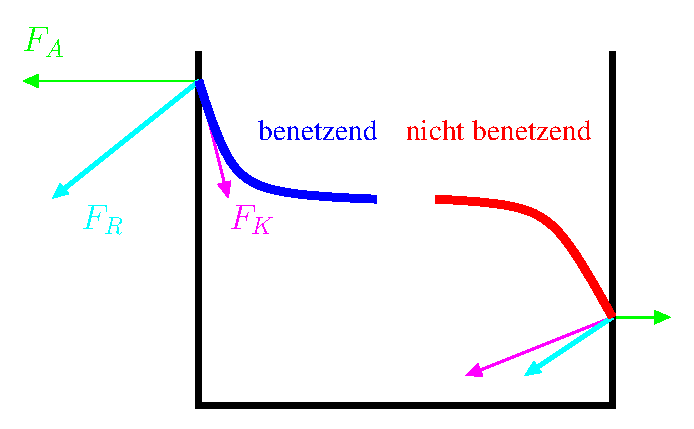
\includegraphics[width=0.4\textwidth]{bilder/benetzen}
      \caption{Wechselwirkungen bei Fl"ussigkeiten}
      \label{abb_benetzen}
   \end{figure}


\item[Fl"ussigkeit--Gas] \textbf{Im Inneren} der Fl"ussigkeit hat das Teilchen
   noch in alle Richtung benachbarte Teilchen und erf"ahrt so aus allen
   Richtungen die gleiche Kraft. In der Summe heben sich die Kr"afte
   weg und es herrscht insgesamt ein \emph{Kr"aftegleichgewicht}.

   \textbf{An der Grenzfl"ache} dagegen haben die Teilchen in Richtung
   der Grenzfl"ache keine Nachbarteilchen mehr. Hier wirken also
   Wechselwirkungen zwischen Teilchen und Nachbar in Richtung Inneres,
   die nicht durch entsprechende Gegenkr"afte \emph{weggehoben}
   werden. Es resultiert eine \emph{Kraft senkrecht zur Oberfl"ache
     nach innen}.

F"ur diese Kr"afte ist die \emph{Koh"asion} verantwortlich.
\end{description} 



Bewegt man ein Teilchen vom Inneren an den Rand, so ist eine Arbeit zu
verrichten: Im Inneren kann man das Teilchen noch ohne Kraft / Arbeit
bewegen; geht es jedoch auf den Rand zu, muss man es gegen eine Kraft
bewegen -- also Arbeit aufwenden. Um die Oberfl"ache $\Delta A$ zu
erzeugen, ben"otigen wir die Energie (die \emph{Arbeit}) $\Delta W$,
um die Teilchen gegen die nach innen wirkende Kraft nach Au"sen zu
bewegen, und es gilt $\Delta W \sim \Delta A$. Wir definieren als Ma"s
daf"ur:
\begin{Def}
   [\index{Oberfl"achenspannung}Oberfl"achenspannung $\sigma$]
   \begin{equation}
      \label{eqn_def_oberflaechenspannung}
      \sigma = \frac{\Delta W}{\Delta A} = \frac{F}{\ell}
   \end{equation}
mit $\ell$ als Randl"ange einer Fl"ussigkeitslamelle.

$\sigma$ hei"st auch "`\textbf{\emph{\index{Spezielle
      Grenzfl"achenenergie}Spezielle
    \index{Grenzfl"achenenergie}Grenzfl"achenenergie}}"'.
\end{Def}
mit der Einheit $[\sigma] =
\frac{\operatorname{J}}{\operatorname{m^2}} =
\frac{\operatorname{N}}{\operatorname{m}}$. Mit "`Lamelle"' ist hier
einfach ein (zweidimensional) gebogener B"ugel gemeint, der einen
zweidimensionalen Fl"ussigkeitsfilm auspannt. Dieser Film "ubt auf
seinen Rahmen die Kraft $F$ aus
Gl. \eqref{eqn_def_oberflaechenspannung} aus, wenn der B"ugel die
L"ange $\ell$ hat. Dabei ist wichtig, dass als Fl"ache $A$ nicht nur
eine Seite der Ebene, sondern beide gez"ahlt werden.

Anschaulich ist die Oberfl"achenspannung ein Ma"s daf"ur, wie
\emph{tragf"ahig} eine Fl"ussigkeit ist.

\begin{Wichtig}
   Die Oberfl"achenspannung ist gleich der
   \index{Oberfl"achenenergie}Oberfl"achen\emph{energie}.
\end{Wichtig}
Eine Fl"ussigkeitsoberfl"ache ist also so "ahnlich wie eine \textbf{elastische
Membran}. Der Unterschied ist aber, dass bei der elastischen Membran $F
\sim d$ ist (mit Auslenkung $d$), wobei bei Fl"ussigkeiten $F = \const$ gilt.



Die Oberfl"achenspannung ist sehr stark \emph{temperaturabh"angig}: Je
w"armer die Fl"ussigkeit ist, desto kleiner ist $\sigma$.



\subsection{Minimalfl"achen}
\label{kap_minimalflachen}


\begin{Wichtig}
   In der Natur bilden sich diejenigen Oberfl"achen mit der geringsten Oberfl"achenenergie.
\end{Wichtig}
\begin{Def}
   [\index{Minimalfl"ache}Minimalfl"ache]
Diese Fl"achen minimaler Oberfl"achenenergie nennen wir Minimalfl"achen.
\end{Def}


\subsubsection{Gekr"ummte Oberfl"achen}
\label{kap_gekrummte-oberflachen}

In einer \textbf{Seifenblase} herrsche der Druck $p_1$, au"serhalb der
Druck $p_0$. Hier konkurrieren nun zwei Kr"afte. Einerseits die Kraft
$F_1$, die aus den Druckverh"altnissen resultiert und nach au"sen
wirkt (weil $p_1 > p_0$):\footnote{Wir tun so, als best"unde die
  Seifenblase aus zwei Halbschalen; Die Kraft senkrecht zu einer
  gedachten Lamelle (einem Umfang) berechnet man mit der Effektiven
  Fl"ache $A = \pi r^2$. W"urde man die komplette Oberfl"ache der
  Halbschale verwenden, so w"urde man auch Kr"afte mit Anteil parallel
  zu $A$ mitnehmen.}
\begin{equation}
   \label{eq:88}
   F_1 = (p_1 - p_0) \cdot A = \Delta p \cdot \pi r^2
\end{equation}
und die Kraft $F_2$, die aus der Oberfl"achenspannung resultiert und
die Blase zusammenh"alt. Dabei haben wir eine Fl"ussigkeitslamelle mit
Rand $\ell = 2 \pi r$, die wir \emph{doppelt} werten, weil wir auch
einen \emph{doppelten} Phasen"ubergang haben: Diese Lamelle hat die
\emph{doppelte} Oberfl"ache, als eine gef"ullte Kugel h"atte.
\begin{equation}
   \label{eq:95}
   F_2 = \sigma \cdot 2\pi r \cdot 2
\end{equation}

Nun herrscht ein \emph{Kr"aftegleichgewicht} zwischen diesen Kr"aften,
also $F_1 = F_2$ und damit
\begin{equation}
   \label{eq:96}
   \Delta p \cdot \pi r^2 =  \sigma \cdot 4\pi r ~\Rightarrow ~ \Delta
   p = \frac{4 \cdot \sigma }{r}
\end{equation}

Wie bereits oben angedeutet ist bei einem  \textbf{Wassertropfen}
durch analoge "Uberlegungen die Formel
\begin{equation}
   \label{eq:97}
   \Delta p = \frac{2 \sigma}{r}
\end{equation}
korrekt, bei der wir nur eine Phasengrenze (au"sen) haben.

\bigskip

Im Allgemeinen gilt:
\begin{Wichtig}
   [\textsc{\index{Young-Laplace-Gleichung}Young-Laplace}-Gleichung] f"ur beliebig geformte Tropfen:
   \begin{equation}
      \label{eq:98}
      \boxed{
\Delta p = \sigma \left ( \frac{1}{r_1} + \frac{1}{r_2} \right ) }
   \end{equation}
$r_1$ und $r_2$ sind die \emph{Hauptkr"ummungsradien} der beiden Schmiegekreise an dem Punkt der Oberfl"ache, an dem die Druckdifferenz gesucht ist. Haupt- bedeutet hier den kleinst- und gr"o"stm"oglichen aller m"oglichen Kr"ummungsradien.
\end{Wichtig}


\subsubsection{Einfluss der Wand auf Minimalfl"ache}
\label{kap_einfluss-wand-auf-minimalflache}


Je nachdem, ob eine Fl"ussigkeit-Gef"a"s-Kombination benetzend ist oder
nicht, "andert sich entsprechend die Oberfl"ache. Wenn wir den Winkel
zwischen Fl"ussigkeitsoberfl"ache und Wand mit $\phi$ bezeichnen, so
erhalten wir f"ur \textbf{benetzende} Fl"ussigkeiten $\phi < 90^\circ$, f"ur
\textbf{vollst"andig benetzende} Fl"ussigkeiten $\phi \approx 0^\circ$
und f"ur \textbf{nicht benetzende} Fl"ussigkeiten $\phi > 90^\circ$.

Zu erkl"aren sind diese Formen durch die resultierenden Vektoren aus
Adh"askon un Koh"asion. In Abb.  \ref{abb_benetzen} sind die
entsprechenden Vektoren eingetragen.

Analog zu unseren "Uberlegungen aus \ref{kap_gekrummte-oberflachen}
m"ussen wir dann n"amlich noch die Kraft $F_R$ mit einbeziehen.



\subsection{Kapillarkr"afte}
\label{kap_kapillarkrafte}

Taucht man d"unne Rohre in eine Fl"ussigkeit so ist die Fl"ussigkeit in
dem Rohr nicht einfach nur senkrecht zur Schwerkraft sondern weist
eine Kr"ummung auf.  Zus"atzlich kann die Fl"ussigkeit sogar noch ein
St"uck in das Rohr (in die Kapillare) hineingezogen werden oder kann
innerhalb der Kapillare eine andere Wasserh"ohe als au"serhalb
erreichen.

Eine \textbf{benetzende} Fl"ussigkeit ist bestrebt, ihren Kontakt zur
Kapillare zu maximieren. Gegen die Kapillarkraft (aus
\eqref{eqn_def_oberflaechenspannung} mit $\ell = 2\pi r$ als Rand der
runden Kapillare)
\begin{equation}
   \label{eq:99}
F_\sigma = \sigma \cdot 2 \pi r   
\end{equation}
wirkt die Schwerkraft
\begin{equation}
   \label{eq:100}
   F_g = m \cdot g = \varrho V \cdot g = \varrho \cdot \pi r^2 h \cdot g
\end{equation}
 Im Gleichgewicht gilt $F_g = F_\sigma$ und damit ergibt sich f"ur die \textbf{Steigh"ohe}:
 \begin{equation}
    \label{eqn_kapillare}
\boxed{    h = \frac{2 \cdot \sigma}{\varrho \cdot r \cdot g} }
 \end{equation}

Betrachte man eine \textbf{nicht benetzende} Fl"ussigkeit, so gilt
Gl. \eqref{eqn_kapillare} ebenso -- nur dass $h$ jetzt nach
\emph{unten} geht; die Herleitung ist v"ollig analog.


\begin{figure}
   \centering
   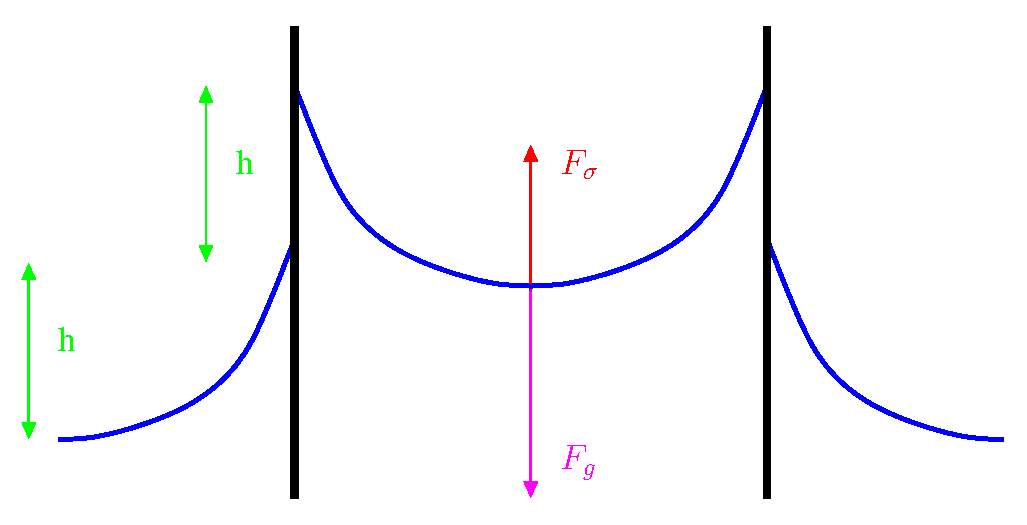
\includegraphics[width=0.6\textwidth]{bilder/kapillarA}
   \hfill
   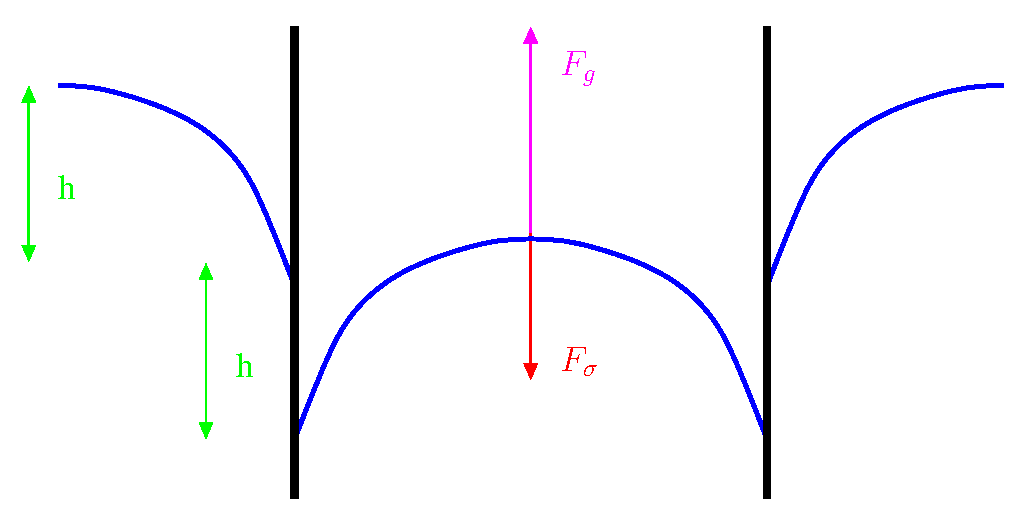
\includegraphics[width=0.3\textwidth]{bilder/kapillarB}
   \caption[Kapillarkräfte]{Kapillarkr"afte: Das rechte Bild ist
     einfach das Spiegelbild des linken, weil die Kapilarkr"afte f"ur
     benetzende und nicht benetzende Fl"ussigkeiten v"ollig analog
     sind.}
   \label{abb_kapillar}
\end{figure}







\section{Ruhende Gase}
\label{kap_ruhende-gase}

Wie Fl"ussigkeiten haben in Gasen die kleinen Teilchen keine feste
Position, daf"ur sind Gase aber komprimierbar.

Analog zur Fl"ussigkeit k"onnen wir hier den \textbf{Stempeldruck} definieren als
\begin{equation}
   \label{eq:63}
   p = \frac{\|\vec F^{(ext)}\|}{A}
\end{equation}
Wobei wir nicht mehr sagen k"onnen, dass eine Kraft senkrecht auf der
Gasoberfl"ache steht. Wir verwenden als Fl"ache $A$ also einfach die
Fl"ache des Stempels, die mit Gas in Kontakt kommt.

Wie wir in der Thermodynamik (Kap. \ref{kap_thermodynamik}) noch
ausf"urhlich sehen werden, gilt f"ur das Verhalten von \emph{idealen} Gasen
\begin{equation*}
   p \cdot V \sim T
\end{equation*}
Wobei \emph{ideale Gase} ein Modell f"ur Gase ist, welches die
Gasteilchen als kleine harte sto"sende Kugeln auffasst und bei kleinen
Dichten eine gute N"aherung darstellt.

\bigskip

Der \textbf{Schweredruck} bei Gasen ist ein wenig schwerer zu fassen:
Weil Gase kompressibel sind, ist 
\begin{Wichtig}
   $\varrho = \varrho(\vec r) = \varrho(h) \neq \const$.
\end{Wichtig}
Wir verwenden statt der eigentlichen Dichte $\varrho$ die
\emph{\index{Teilchendichte}Teilchendichte} $n = n(h) =
\frac{N}{V}$. Es gilt dann mit der idealen Gasgleichung
(s. Kap. \ref{kap_zustandsgroessen-und-gasgleichung}):
\begin{eqnarray}
   \label{eq:64}
\nonumber
   pV &=& NK_BT \\
\nonumber
   p &=& nK_BT
\end{eqnarray}
und f"ur $T = \const$ gilt:
\begin{equation}
   \label{eq:65}
\diff p = K_B T \cdot \diff n   
\end{equation}
Au"serdem gilt f"ur eine kleine Bewegung immernoch\footnote{F"ur
  imkompressible Stoffe gilt $p(h) = \varrho g \cdot h$
  (\ref{eqn_schweredruck}. F"ur einen kleinen Bereich $\diff h$ wollen
  wir nun annehmen, dass Luft auch eine konstante Dichte hat. Das
  "`$-$"' kommt daher, weil der Druck abnimmt ($\diff p < 0$), wenn
  man weiter hoch ($\diff h > 0$) geht.}
\begin{equation}
   \label{eq:66}
   \diff p  = -\varrho(h) \cdot g \cdot \diff h = -nm \cdot g \cdot
   \diff h
\end{equation}
wobei wir $\varrho = n \cdot m$ mit der Teilchenmasse $m$ gesetzt
haben: $n \cdot m = \frac{N \cdot m}{V} = \frac{M}{V} = \varrho$.

Aus Gl. \eqref{eq:65} und Gl. \eqref{eq:66} erhalten wir eine
Differentialgleichung:
\begin{equation}
   \label{eq:67}
    K_B T \cdot \diff n   =  -nm \cdot g \cdot
   \diff h
\end{equation}
Wir l"osen sie durch Trennung der Variablen 
$$
\frac{1}{n} \diff n = \frac{- m \cdot g}{K_B \cdot T} \diff h
$$
und anschlie"sendem Aufintegrieren\footnote{% Dabei ist $n(h =0)$ die
%   Anfgangsbedingung bzw. die Integrationskonstante. Diese wurde auf
%   der rechten Seite weggelassen, weil wir die Integrationskonstannte
%   der Rechten Seite einfach subtrahieren k"onnen und so in $n(h = 0)$
%   "`verstecken"' k"onnen.
  Dabei sind die Grenzen $0$ und $h$. Links wurde verwendet, dass $\ln
  a - \ln b = \ln \frac{a}{b}$ ist. Es ist $n(h = 0) = n_0$.}:
$$
\ln \frac n {n(h = 0)} = \int \frac{1}{n} \diff n = \int \frac{- m \cdot g}{K_B \cdot
  T} \diff h = -\frac{ m \cdot g }{K_B \cdot T}\cdot h
$$
Und um den $\ln$ aufzul"osen verwenden wir die $\exp$-Funktion
\begin{equation}
   \label{eq:68}
n(h) = n_0 \cdot \exp \left ( -\frac{m \cdot g }{K_B \cdot T}\cdot h \right )  
\end{equation}
Und "uber den Zusammenhang $p = n K_B T$ folgt weiter
\begin{equation}
   \label{eq:69}
\boxed{   p(h) = {p_0} \cdot  \exp \left ( -\frac{m \cdot g \cdot h}{K_B \cdot T} \right )  }
\end{equation}
wobei $p_0 = n_0 \cdot K_B T$. Dies ist die
\textbf{\index{Barometrische H"ohenformel}Barometrische H"ohenformel}.









\section{Str"omende Fl"ussigkeiten und Gase}
\label{kap_stromende-flussigkeiten-und-gase}


\begin{Wichtig}
   Wir betrachten \emph{langsam} str"omende Fl"ussigkeiten und Gase mit 
$$
\text{Str"omungsgeschwindigkeit} < \text{Schallgeschwindigkeit}
$$
\end{Wichtig}
Dann k"onnen wir bei Gasen eine konstante Dichte annehmen.

Bei diesen Bedingungen verhalten sich Fl"ussigkeiten und Gase wie
\emph{Fluide} (s. Def. \ref{def_fluid} auf S. \pageref{def_fluid}).

\bigskip
Wir unterscheiden bei Fl"ussigkeiten je nach Reibung drei Typen:
\begin{description}[\setlabelstyle{\bfseries\slshape}]
\item[Z"ahe] Fl"ussigkeiten\\Die Reibung \emph{innerhalb} der
   Fl"ussigkeit dominiert. (Die Str"omungen in diesen Fl"ussigkeiten
   hei"st \textbf{\index{laminar}laminar}.)
\item[Ideale] Fl"ussigkeiten\\Die Reibung ist im Vergleich zur
   kinetischen Energie unbedeutend
\item[Reale] Fl"ussigkeiten\\Die Str"omung ist so schnell, dass
   \emph{Wirbel} entstehen; wir sprechen von einer
   \textbf{\index{turbulent}turbulenten
     Str"omung}. Tr"agheitseffekte der Teilchen sind wichtig.
\end{description}




\subsection{Z"ahe Fl"ussigkeiten}
\label{kap_zahe-flussigkeiten}

Taucht man zwei Platten mit Abstand $d$ in eine Z"ahe Fl"ussigkeit und
will eine davon l"angs mit $v_0$ bewegen\footnote{also stehen die
  Plattenfl"achen \emph{parallel} zur Bewegung}, so braucht man daf"ur
eine Kraft $F_\|$. Diese resultiert daraus, dass die Teilchen in der
unmittelbaren Umgebung der bewegten Platte mitbewegt werden und
ihrerseits ihre "`Nachbarn"' mitbewegen usw.

Die Geschwindigkeit, mit der die einzelnen Wasserteilchen zwischen den
Platten bewegt werden m"ussen, nimmt linear mit dem Abstand zur Platte
ab -- bei der ruhenden Platte sollte er verschwunden sein; wir
sprechen von einem \textbf{\index{lineares
    Geschwindigkeitsprofil}linearen
  \index{Geschwindigkeitsprofil}Geschwindigkeitsprofil}
(s. Abb. \ref{abb_linaers-geschwindigkeisprofil})

Experimentell lassen sich die Zusammenh"ange
$$
F_\| \sim v_0 \text{ , } F_\| \sim A \text{ und } F_\| \sim \frac{1}{d}
$$
ermitteln. Wir definieren nun:
\begin{Def}
   [\index{Viskosit"at}Viskosit"at $\eta$]
Das Ma"s f"ur die \emph{Z"ahigkeit} eines Stoffes:
   \begin{equation}
      \label{eqn_def_viskositaet}
      \eta = \frac{F_\| \cdot d}{A \cdot v_0}
   \end{equation}
\end{Def}
mit der Einheit $[\eta] = \frac{\operatorname{Ns}}{\operatorname{m^2}}
= \operatorname{Pa}\cdot \operatorname{s}$

Da sich die Str"omungsgeschwindigkeit $v$ nicht unbedingt linear
bez"uglich des Abstands $d$ verhalten muss, ist im Allgemeinen diese
Formel richtig:
\begin{equation}
   \label{eq:74}
   \vec F = \eta \cdot A \cdot \frac{\diff \vec v}{\diff d}
\end{equation}
Dabei kann man $\frac{\diff \vec v}{\diff d}$ interpretieren als das
\textbf{Geschwindigkeitsgef"alle}. Also je gr"o"ser dieses Gef"alle ist,
desto gr"o"ser die Kraft...

\bigskip

In einem \textbf{Rohr} wirkt sich das so aus, dass die
Fl"ussigkeitsteilchen in der Rohrmitte am schnellsten Str"omen und die
Geschwindigkeit nach au"sen abnimmt. Dabei nimmt die Geschwindigkeit
quadratisch-proportional nach au"sen hin ab
(s. Abb. \ref{abb_quadratisches-geschwindigkeitsprofil}).

Dabei besteht Reibung nicht nur zwischen Teilchen und Wand, sondern auch
zwischen den Teilchen selbst - sonst w"urden die Teilchen sich ab einer
gewissen Entfernung zur Rohrwand mit der gleichen Geschwindigkeit
bewegen.


% Wir wollen dies n"aher betrachten: Nach Gl. \eqref{eq:74}
% gilt gilt bei infinitissimaler Betrachtung (die Teilchen str"omen in
% $y$-Richtung, das Geschwindigkeitsgef"alle, welches wir betrachten
% wolln, ist in $x$-Richtung) an der linken Seite:
% \begin{equation}
%    \label{eq:72}
%    \diff F_1 = - \eta \cdot \frac{\partial v}{\partial x}|_{\vec r_l}
%    \diff y \diff z
% \end{equation}
% Dies ist die Reibungskraft, die die Fl"ussigkeit erf"ahrt, wenn das
% Fl"ussigkeitsvolumen $\diff V = \diff x \diff y \diff z$ nach rechts
% str"omt. Wie wir aus Gl. \eqref{eq:74} gesehen haben, ist
% die hier herrschende Geschwindigkeitsdifferenz daf"ur entscheidend.

% An der rechten Seite kommen wir formal auf die gleiche Gleichung (mit
% $\vec r_r$ statt $\vec r_l$:
% \begin{equation}
%    \label{eq:73}
%      \diff F_2 =  \eta \cdot \frac{\partial v}{\partial x}|_{\vec r_r}
%    \diff y \diff z
% = \eta \left ( \frac{\partial v}{\partial x}|_{\vec r_l} +
%    \frac{\partial^2 v }{\partial x^2} \diff x \right ) \diff y \diff z
% \end{equation}
% Dabei verwenden wir in der Klammer das linke Gef"alle und addieren
% gewisserma"sen die \emph{Ver"anderung des Gef"alles} im Verlauf der
% $x$-Achse dazu -- daher die zweite Partielle Ableitung.

% Wenn wir nun die resultierenden Reibungskr"afte bestimmen wollen, summieren wir
% \eqref{eq:72} und \eqref{eq:73}:
% \begin{equation}
%    \label{eq:75}
%    \diff F = \diff F_1 + \diff F_2 = \eta \cdot \frac{\partial^2
%      v}{\partial x^2} \underbrace{\diff x \diff y \diff z}_{\diff V}
% \end{equation}




\bigskip

Nach Carl von \textsc{Linné}s \emph{"`Die Natur macht keine Spr"unge"'}
gilt f"ur uns
\begin{Wichtig}
   Geschwindigkeitsprofile sind kontinuierlich.
\end{Wichtig}

\begin{figure}
   \centering
   \subfigure[Linear bei zwei
   Platten]{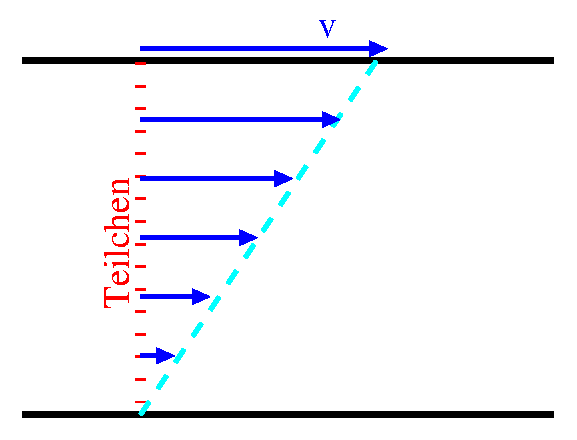
\includegraphics[width=0.3\textwidth]{bilder/lineare-stroemung}\label{abb_linaers-geschwindigkeisprofil}}
\subfigure[Quadratische Str"omung im Rohr]{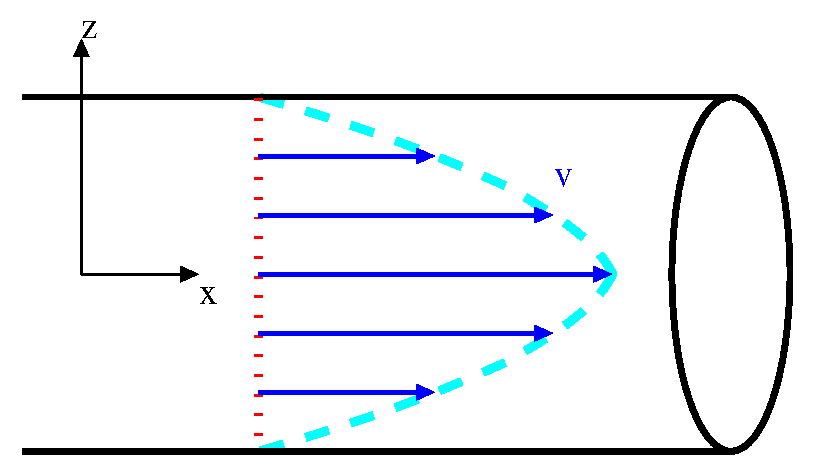
\includegraphics[width=0.3\textwidth]{bilder/quadratische-stroemung}\label{abb_quadratisches-geschwindigkeitsprofil}}
\caption[Geschwindigkeitsprofile von
Flüssigkeiten]{Geschwindigkeitsprofile}
   \label{abb_geschwindigkeitsprofile}
\end{figure}



\subsection{Str"omungsmechanik f"ur z"ahe Fl"ussigkeiten: Laminare Str"omungen}
\label{kap_stromungsmechanik-fur-zahe-flussigkeiten}

\subsubsection{Strom und Widerstand}
\label{kap_strom-und-widerstand}



\begin{Def}
   [\index{Stromst"arke}Stromst"arke $I$] ist die "Anderung des
   (Fl"ussigkeits)Volumens am Ort; also die Differenz aus an- und
   abflie"sender Fl"ussigkei pro Zeiteinheit.
   \begin{equation}
      \label{eqn_def_stromstaerke}
      I = \frac{\Delta V}{\Delta  t} \to \frac{\diff V}{\diff t} =
      \dot V
   \end{equation}
\end{Def}
mit der Einheit $[I] = \frac{m^3}{s}$.

Damit ein Strom flie"st\footnote{die Terminologie ist hier bewusst an
  die der Elektrodynamik angelehnt -- schlie"slich kann man viele
  Zusammenh"ange zwischen diesen beiden Disziplinen feststellen...},
braucht es im betreffenden Leiter einen \emph{Druckunterschied}: Die
Fl"ussigkeit wird dann von Stellen h"oheren Drucks an Stellen
niedrigeren Drucks bewegt: Wenn auf der linken Seite eines Rohres ein
h"oherer Druck herrscht, so kann man sich die Kr"afte auf ein
Wasserteilchen anschauen. Diese m"ussen insgesamt nach rechts zeigen,
weil die Kraft von links (da $F \sim p$ d"urfen wir hier nicht nur von
niedrigerem Druck sondern auch von kleinere Kraft sprechen) schw"acher
ist.

Es gilt der Zusammenhang:
\begin{Wichtig}
   [Stromst"arke -- Druckdifferenz]
Nach \textsc{Haagen-Poiseuille} gilt: Der Stromfluss $I$ ist
proportional zur Druckdifferenz.
\begin{equation}
   \label{eqn_stromstaerke-bei-druckdifferenz}
   I = \frac{p_1 - p_2}{R} = \frac{\Delta p}{R}
\end{equation}
\end{Wichtig}
Dabei hat der Proportionalit"atsfaktor $R$ eine physikalische Bedeutung:
\begin{Def}
   [\index{Str"omungswiderstand}Str"omungswiderstand $R$]
   \begin{equation}
      \label{eq:71}
\boxed{ R = \frac{\Delta p}{I}}
   \end{equation}
\end{Def}
Mit der Einheit $[R] = \frac{\operatorname{Pa} \cdot \operatorname{t}}{\operatorname{m}^3}$.
Er ist abh"angig von 
\begin{itemize}
\item Fl"ussigkeit (also \emph{welche} Fl"ussigkeit str"omt "uberhaupt)
\item Rohrdurchmesser
\item von Geometrie des Rohres (ob es rund, eckig ... ist)
\end{itemize}
Es gilt f"ur ein \textbf{rundes langs Rohr}:
\begin{Wichtig}
   [Gesetz von
   \textsc{\index{Hagen-Poiseuille}\index{Hagen}Hagen-\index{Poiseuille}Poiseuille}]
   Die Stromst"arke ist zur Druckdifferenz proportional (nach
   Gl. \eqref{eq:71}) mit
\begin{equation}
   \label{eq:70}
   \frac{1}{R} = \frac{\pi}{8} \cdot \frac{r^4}{\eta \cdot L}
\end{equation}   
\end{Wichtig}
Wobei $r$ der Radius des Rohres, $L$ die durchstr"omte L"ange und
$\eta$ die Viskosit"at. Man erh"alt es, indem man die Reibungskraft aus
\eqref{eqn_def_viskositaet} mit der Kraft gleichsetzt, welche die
Str"omung erzeugt: $F = A \cdot \Delta p = \pi r^2 \Delta p$.


\subsubsection{Verschaltung von Rohren}
\label{kap_verschaltung-von-rohren}


Wir k"onnen verschiedene Leitungen auf zwei verschiedene Arten
zusammenschalten:
\begin{description}[\setlabelstyle{\bfseries\slshape}]
\item[\index{Reihenschaltung}Reihenschaltung] Die Widerst"ande
   summieren sich, die Stromst"arke muss konstant bleiben:
$$
R_{ges} = \sum_i R_i
$$

\item[\index{Parallelschaltung}Parallelschaltung]
Die reziproken der Widerst"ande addieren sich, die Stromst"arke addiert
sich direkt:
$$I_{ges} = \sum_i I_i$$
$$R_{ges} = \left ( \sum_i \frac{1}{R_i} \right )^{-1}$$
\end{description}
F"ur (analoge) Herleitungen siehe
Kap. \ref{kap_stromkreis-und-schaltungen} auf
S. \pageref{kap_stromkreis-und-schaltungen}.

\begin{figure}
   \centering
\subfigure[Reihenschaltung]{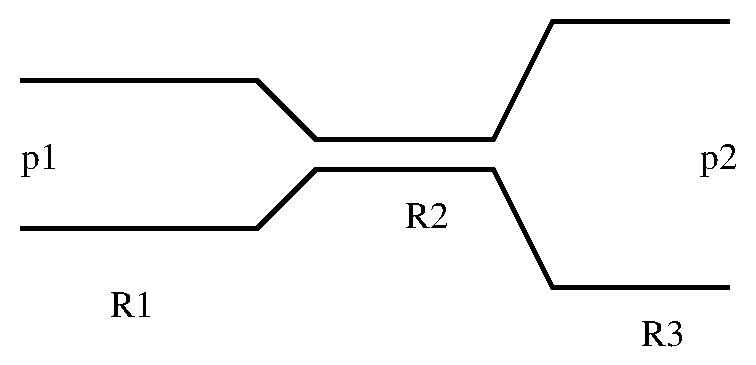
\includegraphics[height=0.1\textheight]{bilder/rohre_reihe}\label{abb_rohre_reihe}}   
\subfigure[Parallelschaltung]{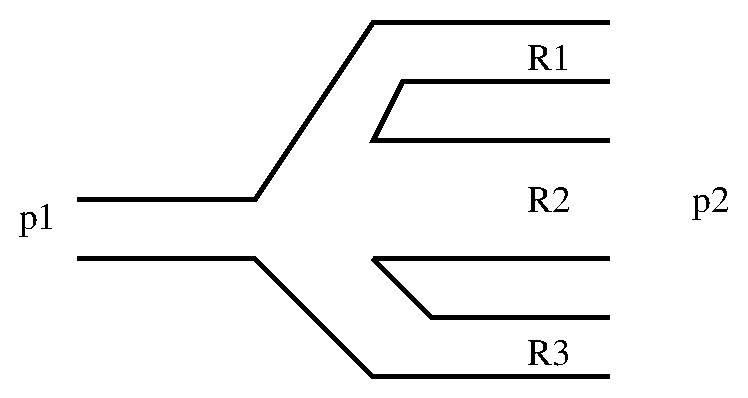
\includegraphics[height=0.1\textheight]{bilder/rohre_parallel}}
   \caption{Schaltungen von Rohren}
   \label{abb_rohre_schaltungen}
\end{figure}


\subsubsection{Festk"orper in Fl"ussigkeit}
\label{kap_festkorper-in-flussigkeit}

\begin{Wichtig}
   [\index{Stokes-Reibung}\textsc{Stokes}-Reibung]
Eine Kugel mit Radius $r$ erf"ahrt die geschwindigkeits($v$)abh"angige Reibung
\begin{equation}
   \label{eq:76}
   F_R = 6 \, \pi \, \eta \, r \cdot v
\end{equation}
\end{Wichtig}
Trotzdem sinken Kugeln mit gro"sem Radius schneller. Das liegt daran,
dass sie einen kleineren Auftrieb haben. Wir betrachten dazu eine
unbeschleunigte Kugel, die mit der konstanten Geschwindigkeit $v_0$ f"allt:
$$
F_G - F_A - F_R = 0 ~ ~\Rightarrow F_G - F_A = F_R
$$
wobei wir die nach unten weisenden Kr"afte als positiv ansehen. Setzen
wir \eqref{eq:61} und \eqref{eq:76} ein, erhalten wir:
\begin{eqnarray*}
   \label{eq:77}
   \varrho_\text{Kugel} \cdot g \cdot V - \varrho_\text{Fl} \cdot g
   \cdot V &=& 6\pi\eta r \cdot v_0 \\
   (\varrho_\text{Kugel} - \varrho_\text{Fl}) \cdot g
   \cdot \frac{4}{3}\pi r^3  &=& 6\pi\eta r \cdot v_0 
\end{eqnarray*}
\begin{equation}
   \label{eq:78}
   v_0 =  (\varrho_\text{Kugel} - \varrho_\text{Fl}) \cdot g \cdot
\frac{4 \pi r^3}{3 \pi \eta r} = (\varrho_\text{Kugel} -
\varrho_\text{Fl}) \cdot g \cdot \frac{4 r^2}{3 \eta}
\end{equation}
also der Zusammenhang
\begin{equation}
   \label{eq:79}
   v_o \sim \frac{r^2}{\eta}
\end{equation}

Diesen Sachverhalt k"onnen wir f"ur die \emph{Viskosit"atsbestimmeung} mit
\emph{\index{Kugelfallviskosimetern}Kugelfallviskosimetern} verwenden;
hier kann man aus $v$ $\eta$ errechnen.

\begin{Def}
   [\textsc{Newton}'sche Fl"ussigkeit]
Wir nennen eine Fl"ussigkeit \textsc{Newton}'sch, wenn gilt
\begin{equation}
   \label{eq:80}
   v \sim \frac{1}{\eta}
\end{equation}
\end{Def}









\subsection{Ideale Fl"ussigkeit}
\label{kap_ideale-flussigkeit}

Wo bei den z"ahen Fl"ussigkeiten die Reibungskr"afte noch ausschlaggebend
waren, k"onnen wir diese jetzt vernachl"assigen.

Wir betrachten bspw. ein gef"ulltes Rohr mit Druckunterschied an den
beiden Enden. Die Fl"ussigkeit wird vom Bereich hohen Drucks zum
Bereich niedrigen Drucks flie"sen. Wenn jetzt aber zwischen den beiden
Enden noch eine \emph{Verj"ungung} im Rohr ist, so wird hier der Druck
\emph{kleiner} sein, als an den beiden Rohrenden
(vgl. Abb. \ref{abb_rohr_verjuengung}). Trotzdem wird die Fl"ussigkeit
weiterflie"sen.

Wir betrachten dazu ein bestimmtes Volumen $\Delta  V$ in den drei
verschiedenen Rohrabschnitten. Die \emph{Stromst"arke} muss dabei
konstant bleiben: 
\begin{equation}
   \label{eq:81}
   I = \frac{\Delta V}{\Delta t} = \frac{\diff V_i}{\diff t} = \frac{A_i \cdot \diff s_i}{\diff t} =
A_i \cdot v_i = \const
\end{equation}
Daraus k"onnen wir folgern:
\begin{itemize}
\item je kleiner das Rohrdurchmesser $A_i$ ist, desto gr"o"ser ist die
   entsprechenden Geschwindigkeit $v_i$.
\item Die Kinetische Energie "andert sich beim Fluss:
   \begin{equation}
      \label{eq:82}
      \Delta E_{kin} = \frac{1}{2} \underbrace{\varrho \cdot \Delta
        V}_{\Delta M} ( v_2^2 - v_1^2 )
   \end{equation}
\end{itemize}

Andererseits m"ussen wir beachten, dass beim Str"omen die Arbeit
("`Volumenarbeit"') verrichtet wird:
\begin{equation}
   \label{eq:83}
   W =  \int F \diff s \stackrel{\const}{=} F \cdot s = \underbrace{p \cdot A}_F
   \cdot s = p \cdot V
\end{equation}
und damit
\begin{equation}
   \label{eq:84}
   \Delta W = (p_1 - p_2) \cdot \Delta V
\end{equation}
dies entspricht einer \textbf{potentiellen} Energie: Die Energie, die
aufgebracht werden muss, um den Druck von $p_1$ auf $p_2$ zu
"andern. Nach dem Energieerhaltungssatz muss nun gelten $\Delta W =
\Delta E_{kin}$ und mit Gl. \eqref{eq:82} und \eqref{eq:84}:
\begin{equation}
   \label{eq:85}
   \frac{1}{2} \underbrace{\varrho \cdot \Delta
     V}_{\Delta M} ( v_2^2 - v_1^2 )  = (p_1 - p_2) \cdot \Delta V   
\end{equation}
und man erh"alt durch Umformung:
\begin{equation}
   \label{eq:86}
  \frac{1}{2} \cdot \varrho \cdot v_2^2 + p_2 = \frac{1}{2} \cdot
   \varrho \cdot v_1^2 + p_1 
\end{equation}
und diese Formel ist an beliebigen Stellen g"ultig! Wir bezeichnen sie
als:
\begin{Wichtig}
   [\textsc{\index{Bernulli-Gleichung}Bernulli}-Gleichung] f"ur
   horizontal str"omende, ideale Fl"ussigkeiten:
   \begin{equation}
      \label{eq:87}
        \underbrace{\frac{1}{2} \cdot \varrho \cdot
          v^2}_\text{Staudruck} + \underbrace{p}_\text{hydrostatischer
        Druck} =  p_{ges} = \const
   \end{equation}
\end{Wichtig}
Dabei ist der hydrostatische Druck der von einem Barometer messbare
Druck.
\begin{figure}
   \centering
   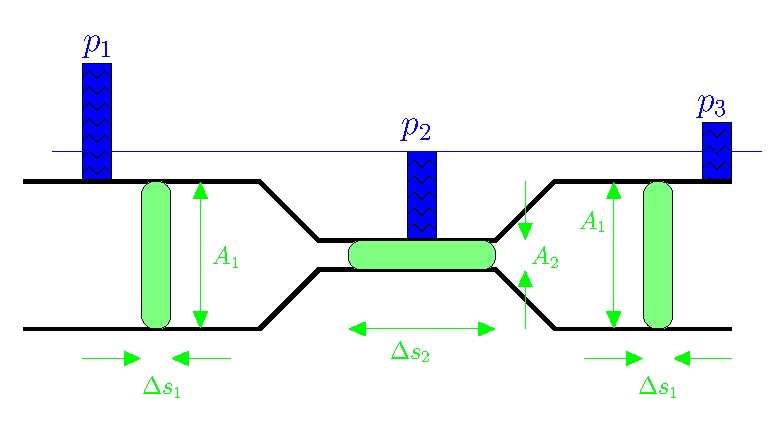
\includegraphics[width=0.7\textwidth]{bilder/rohr_verjuengung}
   \caption[Ideale Flüssigkeit in untersch. dickem Rohr]{Ein Rohr
     mit Verj"ungung, gef"ullt mit einer idealen Fl"ussigkeit. Gr"un
     ist ein einheitliches Volumen in den Drei Rohrabschnitten, blau
     ist der Druck -- also eine Wassers"aule, die man im Experiment
     sehen k"onnte.}
   \label{abb_rohr_verjuengung}
\end{figure}



\subsection{Anwendungen bei idealen Fl"ussigkeiten}
\label{kap_anwendungen-bei-idealen-flussigkeiten}

Ein paar Anwendungen:
\begin{Beispiel}
\begin{enumerate}[(i):]
\item \textbf{\index{Zerst"auber}Zerst"auber /
     \index{Wasserstrahlpumpe}Wasserstrahlpumpe}: Durch ein Rohr wird
   ein Fluid geschickt. An einer Verj"ungung ist ein zweites Rohr
   angeschlossen. An dessen Ende setzt man die zu zerst"aubende
   bzw. anzupumpende Substanz. Dadurch, dass das Fluid an der engeren
   Stelle schneller flie"sen muss, ist der Druck hier sehr klein und
   die Stoffe werden angesaugt und in den allgemeinen Strom des Rohres
   beigemischt.

\item \textbf{\index{Pradoxon}Pradoxon}:
%  Wenn man einen Ball unten an eine Platte h"alt
%    und \emph{von oben} Luft herunterbl"ast, f"allt der Ball nicht
%    herunter: Die Luft umstr"omt den Ball und muss
   Setzt man einen Ball in einen umgest"ulpten Trichter und pustet von
   oben in diesen Trichter, so f"allt der Ball nicht herunter (wenn er
   leicht genug ist).

   Die Luft Umstr"omt den Ball und braucht dabei eine l"angere Strecke
   (weil der Ball rund ist). Folglich ist sie schneller und damit ist
   hier der Luftdruck klein. Zwischen Trichter und Ball ist der
   Luftdruck so klein, dass der Ball an die Trichterwand gezogen wird.

\item \textbf{\index{Bananenflanke}Bananenflanke}: Wenn ein Ball von
   einer schiefen Ebene in ein Wasserbecken f"allt, so wird er hier
   nicht seinen Weg geradlienig fortsetzen, sondern eine krumme Bahn
   "`schwimmen"' (vgl. Abb. \ref{abb_banane}).

   Die Fl"ussigkeitsteilchen nahe der Kugel bewegen sich im Wasser mit
   der Kugel -- sie hat noch eine Rotation von ihrem Weg auf der
   Schiefen Ebene. Auf der \emph{rechten} Seite bewegen sich die
   Molek"ule bez"uglich der Kugel besonders schnell, weil sich hier die
   Rotation der Kugel und ihr Herabsinken addieren\footnote{Wenn die
     Kugel herabsinkt, so fallen die Fluidteilchen um sie herum
     \emph{relativ nach oben}.}. Auf dieser Seite ist also $v$ gro"s
   und damit $p$ klein: Die Kugel wird also nach rechts
   "`gesaugt"'. (s. Def. \ref{def_magnuskraft})


\item \textbf{\index{Golfball}Golfb"alle}: Die kleinen Vertiefungen in
   den Golfb"allen sorgen daf"ur, dass der Magnus-Effekt hier
   besonders stark auftritt. Da der Golfschl"ager den Ball schr"ag
   abschie"st und in Rotation versetzt, sorgt so der Magnus-Effekt
   beim Golfball daf"ur, dass dieser nach oben gezogen wird und damit
   weiter fliegt.
\end{enumerate}
\end{Beispiel}

\begin{Def}
   [\index{Magnuskraft}\textsc{Magnus}kraft] 
\label{def_magnuskraft}Die Querkraft, die ein
   rotierender runder K"orper in einem Fluid bzw. einer Str"omung
   erf"ahrt.
\end{Def}

\begin{figure}
   \centering
   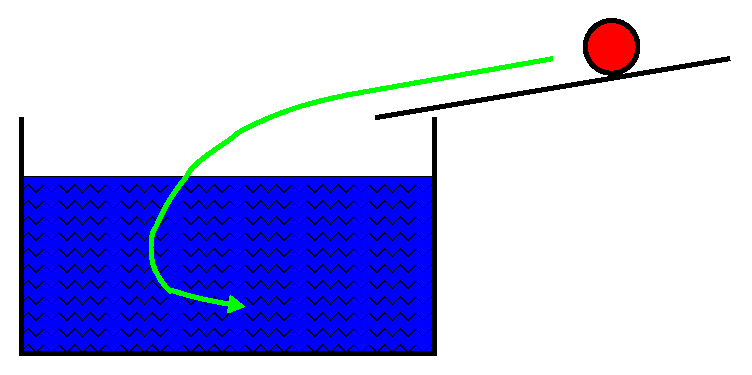
\includegraphics[width=0.5\textwidth]{bilder/banane_traj}
\hfill
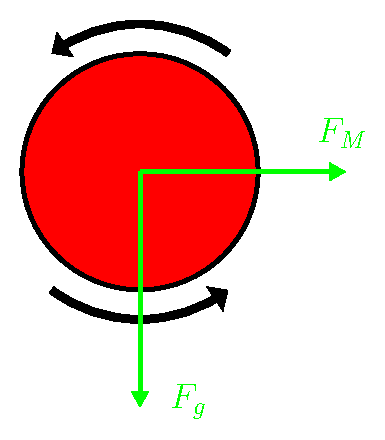
\includegraphics[width=0.3\textwidth]{bilder/banane_vekt}
   \caption{Bananenflanke: Trajektorie und Vergr"o"serung der Kugel}
   \label{abb_banane}
\end{figure}








\subsection{Reale Fl"ussigkeiten}
\label{kap_reale-flussigkeiten}

Wir behandeln schnelle Str"omungen; hier sind die ausschlaggebenden
Gr"o"sen die \emph{Tr"agheitseffekte}. (Die Tr"agheitskr"afte sind weit
gr"o"ser als die Reibungskr"afte.)


Bei kleinen Geschwindigkeiten haben wir geordnete, \emph{laminare}
Str"omungen (vgl. Abb. \ref{abb_geschwindigkeitsprofile}) -- bei
gro"sen Geschwindigkeiten kann es bei realen Fl"ussigkeiten zu
\emph{\index{Turbulenz}turbulenten Str"omungen} kommen, bei denen sich
\emph{\index{Wirbel}Wirbel} bilden.

Diese \textbf{Wirbelbildung} hinter einem Hindernis kann man einfach
dadurch erkl"aren, dass wenn ein Fl"ussigkeitsvolumen an dem Hindernis
vorbeiwandert, seine "au"seren Teilchen direkt am Hindernis
anliegen. Hier wirkt also eine gro"se Reibungskraft auf die
Teilchen. Je weiter weg vom Hindernis -- also "`im Inneren"' des
Fl"ussigkeitsvolumens -- ist die Reibung kleiner, und damit die
Geschwindigkeit gr"o"ser. Da also nahe am Hindernis die
Teilchengeschwindigkeit klein und weit davon entfernt gro"s ist, wird
das Fl"ussigkeitsvolumen eine Rotation bekommen. Durch den
\emph{\textsc{Magnus}-Effekt} (s. Def. \ref{def_magnuskraft}) wird es
dann schlie"slich hinter das Hindernis gezogen: Ein erster kleiner
Wirbel ist entstanden.

Bei gro"sen Geschwindikgeiten kann es nun auch dann zu Wirbeln kommen,
wenn gar keine Hindernisse im Weg waren: Das kommt dann von der
Geschwindigkeits\emph{fluktuation} der Teilchen des
Fl"ussigkeitsvolumens.

\bigskip

Um zu entscheiden, ob eine Str"omung turbulent oder laminar ist, m"ussen
wir unterscheiden ob Tr"agheits- (turbulent) oder Reibungskr"afte
(laminar) die Oberhand haben; daf"ur untersuchen wir den Quotienten
\begin{equation*}
   \label{eq:89}
   \frac{F_\text{Tr"agheit}}{F_\text{Reibung}}
\end{equation*}
und untersuchen die beiden Kr"afte separat:
\begin{description}[\setlabelstyle{\bfseries\slshape}]
\item[Tr"agheit] Ein bewegter K"orper "ubertr"agt Impuls auf Fl"ussigkeit:

Eine Kugel mit Radius $a$ "uberstreicht in $\diff t$ das Volumen $A
\cdot \diff s$. 
Dabei gilt f"ur die Bewegte Menge (Masse) Fl"ussigkeit:
\begin{equation}
   \label{eq:90}
   \frac{\diff m}{\diff
  t} = \varrho \cdot \frac{\diff V}{\diff t} = \varrho \cdot A \cdot
\frac{\diff s}{\diff t} = \varrho \cdot A \cdot v
\end{equation}
Nun muss jedes Teilchen dieser Masse wegbewegt werden. Da wir hier die
Reibung noch au"sen vor lassen, ist dazu lediglich die (Tr"agheits)Kraft 
\begin{equation}
   \label{eq:92}
      F = \frac{\diff p}{\diff t} = \dot p
\end{equation}
 n"otig mit $p = m \cdot v$.
Es gilt:
\begin{equation}
   \label{eq:91}
   \frac{\diff p}{\diff t} = \frac{\diff m \cdot v}{\diff t} +
   \frac{m \cdot \diff v }{\diff t}
\end{equation}
Da wir die Geschwindigkeit hier als konstant ansehen, verschwindet der
zweite Summand. Setzen wir nun also Gl. \eqref{eq:90} in \eqref{eq:91}
und dies in \eqref{eq:92} ein, so erhalten wir:
\begin{equation}
   \label{eq:93}
   F = F_\text{Tr"agheit} = \varrho \cdot A \cdot v^2 = \varrho \cdot
   \pi a^2 \cdot v^2
\end{equation}


\item[Reibung] Die Reibung innerhalb der Fl"ussigkeit ist nach
   Gl. \eqref{eq:76}:
   \begin{equation*}
      F_\text{Reibung} = 6 \pi \eta a \cdot v
   \end{equation*}
   Dabei gilt diese Formel \emph{eigentlich} f"ur ein K"ugelchen des
   Radius $a$. \emph{Eigentlich} m"ussten wir hier f"ur die Herleitung
   die unhandliche
   \textsc{\index{Navier-Stokes-Gleichung}Navier-Stokes}-Gleichung
   verwenden;
   \begin{equation}
      \label{eq:21}
      \varrho \left ( \frac{\partial }{\partial t} + \vec v \cdot \vec
         \nabla \right ) \vec v = -\vec\nabla p + \varrho \cdot \vec g
            + \eta \cdot  \Delta \vec v
   \end{equation}
   wobei $\vec v$ die Bewegung der Teilchen und $\vec g$ die
   Schwerebeschleunigung darstellt. (Die rechte Seite der Gleichung
   beschreibt Kr"afte (das $\Delta$ ist der \emph{Laplace}-Operator)
   und die linke Seite die dadurch hervorgerufene Bewegung.) F"ur
   unsere Zwecke ist die empirisch gefundene \textsc{Stokes}-Reibung
   aber gut genug. (Deshalb haben wir aber in \eqref{eq:94} rechts
   auch keine \emph{Gleichheit}, sondern nur eine \emph{Proportionalit"at}.)
\end{description}
Nun k"onnen wir also den Quotienten bilden:



\begin{Def}
   [\textsc{\index{Reynoldszahl}Reynolds}zahl]
Ein Ma"s, ob eine Str"omung laminar ($R_e < 1$) oder turbulent ($R_e \gg
1$) ist:
\begin{equation}
   \label{eq:94}
R_e =   \frac{F_\text{Tr"agheit}}{F_\text{Reibung}} 
=
    \frac{\varrho \cdot d \cdot v}{\eta} 
\sim
 \frac{\varrho \cdot \pi a^2 \cdot v^2}{6 \pi \eta a v}
\end{equation}
hier ist $d$ der Str"omungsdurchmesser des Gegenstandes.
\end{Def}

Hier flie"st ein: Wenn die Reibung wichtiger ist, ist der Nenner
gr"o"ser, damit die Zahl $R_e$ klein ($R_e < 1$) und damit k"onnen wir
die Betrachtungen aus Kap. \ref{kap_zahe-flussigkeiten}
verwenden. Wenn dagegen die Tr"agheitskr"afte einen entscheidenden
Einfluss bekommen, so wird der Bruch sehr gro"s und wir erhalten
Wirbel.

Da aber auch der Radius $a$ in der Formel auftaucht, k"onnen wir sagen,
dass f"ur kleine $a$ im Normalfall $R_e < 1$.


\begin{Beispiel}
   \textbf{Ruder vs Propeller:} Wenn sich ein kleines Objekt ($a$
   klein \Impl $R_e$ klein \Impl z"ahe Fl"ussigkeit) in einer
   Fl"ussigkeit fortbewegen will, so kann es nicht "`rudern"', weil es
   beim Vorziehen der Ruder wieder die Strecke zur"uckbewegt w"urde,
   die es beim Zur"uckziehen der Ruder vorw"arts gekommen ist. Das
   kleine Objekt braucht einen \emph{Propeller}.

   \textbf{Im Windkanal:} Damit man ein Modell unter realistischen
   Bedingungen testen kann, muss man in Windkan"alen den Druck (und
   damit die Dichte $\varrho$) so anpassen, dass die
   \textsc{Reynolds}zahl in Experiment und Realit"at "ubereinstimmt.
\end{Beispiel}
























%%%%%%%%%%%%%%%%%%%%%%%%%%%%%%%%%%%%%%%%%%%%%%%%%%%%%%%%%%%%%%%%%

%%%%%%%%%%%%%%%%%%%%%%%%%%%%%%%%%%%%%%%%%%%%%%%%%%%%%%%%%%%%%%%

%%%%%%%%%%%%%%%%%%%%%%%%%%%%%%%%%%%%%%%%%%%%%%%%%%%%%%%%%%%%%%%%



